\documentclass[11pt,conference,onecolumn]{IEEEtran}
\IEEEoverridecommandlockouts
% The preceding line is only needed to identify funding in the first footnote. If that is unneeded, please comment it out.
\usepackage[utf8]{inputenc}
\usepackage[T1]{fontenc}
\usepackage{amsthm}
\usepackage{amsmath,amssymb,amsfonts}
\usepackage{cite}
\usepackage{algorithmic}
\usepackage{multirow}
\usepackage{graphicx}
\usepackage{textcomp}
\usepackage{xcolor}
\usepackage{setspace}
\usepackage{verbatimbox}
\usepackage{thmtools}
\usepackage{float}

\declaretheoremstyle[spaceabove=6pt, spacebelow=6pt,headfont=\normalfont\bfseries,notefont=\mdseries, notebraces={(}{)},bodyfont=\normalfont,postheadspace=0.6em,
headpunct=:]{mystyle}
\declaretheorem[style=mystyle, name=Hypothesis, preheadhook={\renewcommand{\thehyp}{H\textsubscript{\arabic{hyp}}}}]{hyp}

\usepackage{cleveref}
\crefname{hyp}{hypothesis}{hypotheses}
\Crefname{hyp}{Hypothesis}{Hypotheses}

\def\BibTeX{{\rm B\kern-.05em{\sc i\kern-.025em b}\kern-.08em
    T\kern-.1667em\lower.7ex\hbox{E}\kern-.125emX}}
\begin{document}

\title{Sorting algorithms: how are they affected by memory faults?}

\author{\IEEEauthorblockN{Alexandro Vladno}
\IEEEauthorblockA{\textit{Centre for Informatics and Systems} \\
\textit{University of Coimbra}\\
Coimbra, Portugal \\
alexandro.vladno@gmail.com}
\and
\IEEEauthorblockN{Fabiano Papaiz}
\IEEEauthorblockA{\textit{Centre for Informatics and Systems} \\
\textit{University of Coimbra}\\
Coimbra, Portugal \\
fabianopapaiz@gmail.com}
\and
\IEEEauthorblockN{Leo Moreira Silva}
\IEEEauthorblockA{\textit{Centre of Informatics and Systems} \\
\textit{University of Coimbra}\\
Coimbra, Portugal \\
leo.moreira@me.com}
}

\maketitle

\begin{abstract}
This document is a model and instructions for \LaTeX.
This and the IEEEtran.cls file define the components of your paper [title, text, heads, etc.]. *CRITICAL: Do Not Use Symbols, Special Characters, Footnotes, 
or Math in Paper Title or Abstract.
\end{abstract}

\begin{IEEEkeywords}
component, formatting, style, styling, insert
\end{IEEEkeywords}

\onehalfspacing

\section{Introduction}
Technology is deeply introduced in people's quotidian supporting a massive number of tasks, for example: searching for a shared car, surfing on the web, sending a message to someone, automating the company's production or using the company's software. Nevertheless, most people don't know that devices are continually dealing with memory failures, faults and errors. These devices were made with large and inexpensive memories, which are also error-prone \cite{Finocchi2004}.

Software behavior may be affected by the problems mentioned before, especially those from memory. We have a memory fault when the correct value that should be stored in a memory location gets altered because of a soft failure. In particular, the content of a location can change unexpectedly, i.e., faults may happen at any time: real memory faults are indeed highly dynamic and unpredictable \cite{Hamdioui2003}.

In the beginning steps of software development, the designer has a general idea of the structure and functions. For each one of these, some algorithms will be produced or used. In the following stages, the outcome software (and its algorithms) will be tested and, then, delivered to the user. Different kinds of algorithms could be written or used in the software, and one of these is the sorting algorithms.

A good algorithm is that which gives satisfactory results for every range of data set. Sorting is a fundamental concept and important for solving other problems like is prerequisite for Binary Search. Sorting is often used in a large variety of critical applications and is a fundamental task that is used by most computers \cite{NitinArora}.

In this paper, we present a discussion about how these sorting algorithms, particularly Quicksort, Mergesort, Insertion Sort and Bubblesort, are affected by memory faults.

\subsection{Memory Faults}

Even the best digital system, with high-quality components and design techniques, may not be infallible to faults. Despite the title of this subsection, when the entire digital system (or software) is considered, there are three terms for computing fault and they have different meanings: failure, fault and error \cite{Nelson1990}. 

\begin{itemize}
    \item \textit{Error}: An error is a manifestation of a fault in a system, in which the logical state of an element differs from its intended value. An error occurs for a particular system state and input when an incorrect next state and/or output results.
    \item \textit{Fault}: A fault is an anomalous physical condition. Causes include design errors, manufacturing problems, damage, fatigue, or other deterioration. Faults resulting from design errors and external factors are especially difficult to model and protect against because their occurrences and effects are hard to predict. A fault in a system does not necessarily result in an error;
    \item \textit{Failure}: A failure denotes an element's inability to perform its functions because of error in the element itself or its environment, which in turn are caused by various faults;
\end{itemize}

\section{Sorting Algorithms}

Sorting algorithms are widely used in many aspects of data processing, information searches, business finance, computer encryption, etc. This work uses four sorting algorithms: quicksort, mergesort, insertionsort, and bubblesort. In the following subsections, we'll give an overview of them.

\subsection{Quicksort}

Quicksort algorithm, created by Hoare \cite{Hoare1962}, is considered as one of the fastest and best sorting algorithms \cite{Wang2011}. The algorithm is based on the paradigm of divide and conquer.

This algorithm has a execution time of $\theta(n^2)$ in the worst case over \textit{n} numbers as input. Despite that execution time, quicksort is often the best option for sorting because of its remarkable average efficiency: $\theta(n lg n)$ \cite{Cormen2009}.

The basic steps of this algorithm are \cite{Wang2011}:
\begin{itemize}
    \item Pick an element, which is called a pivot, from the list waiting to be sorted;
    \item Perform partition operation to realize that all elements in the list with values smaller than the pivot came before the pivot. Otherwise, all elements in the list with values bigger than the pivot come after it (elements which are equal to pivot can go either way). After this partition, the pivot is in the final position of the list;
    \item Recursively sort the sub-list of smaller elements and the sub-list of the bigger elements.
\end{itemize}

\subsection{Mergesort}

Mergesort was invented by John Von Newman and is one of the most elegant algorithms to appear in the sorting literature. It is the first sorting algorithm to have $\theta(n lg n)$ execution time bound. It is important to observe that this algorithm spends a lot of time on data transfer operations. In fact, standard Mergesort incurs about 2n data move operations \cite{Abhyankar2011}.

Conceptually, Mergesort works as follows \cite{Abhyankar2011}:
\begin{itemize}
    \item Divide the unsorted array into two sub arrays of about half the size;
    \item Sort each sub array recursively;
    \item Merge the two sub arrays back into one array.
\end{itemize}

\subsection{Insertionsort}

This algorithm sorts the array by shifting the elements one at time. It is efficient in sorting a small number of elements. The overall execution time of this algorithm is $\theta(n^2)$ \cite{Cormen2009}. The basic sorting steps are:
\begin{itemize}
    \item If there are more than one element, pick the next element;
    \item Compare with all the elements in sorted sub-list;
    \item Shift all the elements in sorted sub-list that is greater than the value to be sorted;
    \item Insert the value;
    \item Repeat until list is sorted.
\end{itemize}

\subsection{Bubblesort}

The bubble sort is the oldest and simplest sorting method in use. It works by comparing each item in the list with the item next to it, and swapping them if required. The algorithm repeats this process until it makes a pass all the way through the list without swapping any items (in other words, all items are in the correct order) \cite{Mansotra2011}.

Table \ref{table1} below shows the time complexity comparison between the sorting algorithms presented. The \textit{n} is the number of input elements.

\begin{table}[htbp]
    \caption{Sorting algorithms complexity time comparison \cite{Prajapati2017}}
    \begin{center}
    \begin{tabular}{|c|c|c|c|}
    \hline
    \multirow{2}{*}{\textbf{Algorithm}}&\multicolumn{3}{|c|}{\textbf{Time Complexity}} \\
    \cline{2-4} 
    & \textbf{\textit{Best Case}} & \textbf{\textit{Average Case}}& \textbf{\textit{Worst Case}} \\
    \hline
    Bubblesort & $O(n^2)$ & $O(n^2)$ & $O(n^2)$ \\
    Insertionsort & $O(n)$ & $O(n^2)$ & $O(n^2)$ \\
    Quicksort & $O(nlgn)$ & $O(nlgn)$ & $O(n^2)$ \\
    Mergesort & $O(nlgn)$ & $O(nlgn)$ & $O(nlgn)$ \\
    \hline
    \end{tabular}
    \label{table1}
    \end{center}
\end{table}

\section{Materials and Methods}

We first state our problem, then describe our data, showing all its characteristics. Then, we provide our hypothesis, define the setup, and perform the testing. Finally, we collect and perform data analysis.

\subsection{Problem Statement}

As introduced in the first section of this paper, sorting is a fundamental concept and essential for solving other problems. The content of memory location can change unexpectedly, i.e., faults may happen at any time. Considering this, the main objective of this work is to design experiments to answer the following question: \textit{How are sorting algorithms affected by memory faults?}

\subsection{Variables}

For this experimental study, we assume that the independent and dependent variables are as shown in Table \ref{table-independent-variables} and Table \ref{table-dependent-variables} below:

\begin{table}[H]
    \caption{Independent variables.}
    \begin{center}
    \begin{tabular}{|l|l|}
    \hline
    \textbf{Variable} & \textbf{Description} \\
    \hline
    Probability of failure & Probability of a fault to occur \\
    \hline
    Array size & Size of the array of integers to be sorted \\
    \hline
    Sorting algorithm & Algorithm used to sort the array \\
    \hline
    \end{tabular}
    \label{table-independent-variables}
    \end{center}
\end{table}

\begin{table}[H]
    \caption{Dependent variables.}
    \begin{center}
    \begin{tabular}{|l|l|}
    \hline
    \textbf{Variable} & \textbf{Description} \\
    \hline
    Largest subarray size & Size of the largest sorted subarray produced under the memory fault \\
    \hline
    Percentage of largest subarray size & Percentage of \textit{largest subarray size} related to \textit{array size} independent variable \\
    \hline
    Unordered elements quantity & Quantity of elements out of position after sorting algorithm execution. Adapted of the \\ & \textit{k-unordered sequence} measure of disorder defined in \cite{Ferraro-Petrillo2009} \\
    \hline
    Percentage of unordered elements quantity & Percentage of \textit{unordered elements quantity} related to \textit{array size} independent variable \\
    \hline
    \end{tabular}
    \label{table-dependent-variables}
    \end{center}
\end{table}

\subsection{Hypothesis}

The set of hypothesis defined to test and draw some conclusions about this experiment are listed below. The confidence degree defined for hypothesis testing was 95\% ($\alpha = 0.05$ and $\alpha - 1 = 0.95$).

\begin{itemize}
    \item \textbf{Hypothesis 1:} For a given probability of failure and array size, tested algorithms will produce a different percentage of unordered elements quantity.
    \item \textbf{Hypothesis 2:} For a given probability of failure and array size, tested algorithms will produce a different percentage of the largest subarray size.
    \item \textbf{Hypothesis 3:} For each algorithm, the array size and probability of failure have a significative impact on the percentage of unordered elements quantity.
    \item \textbf{Hypothesis 4:} For each algorithm, the array size and probability of failure have a significative impact on the percentage of the largest subarray size.
\end{itemize}

% \setcounter{hyp}{-1}
% \begin{hyp}[Test hypothesis] \label{hyp:a}There is no difference in memory faults between tested algorithms.\end{hyp}
% \begin{hyp} \label{hyp:b}There are differences in memory faults between tested algorithms. \end{hyp}
% \begin{hyp} \label{hyp:c} An algorithm is better than others considering all dependent variables. \end{hyp}

% \begin{hyp} \label{hyp:d} ... \end{hyp}

\subsection{Experimental Setup}

To conduct the proposed study, we define the values of the independent variables, as shown in Table \ref{table-independent-variables-values}:

\begin{table}[H]
    \caption{Values of the independent variables.}
    \begin{center}
    \begin{tabular}{|c|c|}
    \hline
    \textbf{Variable} & \textbf{Values} \\
    \hline
    Probability of failure & 1\%, 2\% and 5\% \\
    \hline
    Array size & 100, 1000 and 10000 \\
    \hline
    Sorting algorithm & Bubblesort, Quicksort, Mergesort and Insertion sort \\
    \hline
    \end{tabular}
    \label{table-independent-variables-values}
    \end{center}
\end{table}

Based on these variables, we ran an existing script \textit{gen.py} to produce input files. We define that our sample was composed by 30 input files for a given combination of the probability of failure and array size. So, considering this, we ran 30 times for each combination of these independent variables, producing 30 inputs, totalizing 270 files. Figure \ref{fig-input-file-example} shows an example of produced input files:

% \begin{itemize}
%     \item A script that generates input files;
%     \item Four files, one for each of those algorithms: quicksort, bubblesort, insertion sort, and mergesort, that are used to sorting the input data;
% \end{itemize}

\begin{verbbox}[\mbox{}]
0.01 100 9 48 37 6 26 7 24 44 17 50 48 30 49 33 22 13 42 29 39 13 19 13 9 28 
34 1 33 27 14 45 48 40 11 17 6 50 9 44 20 16 37 45 23 14 38 29 10 49 44 46 35
45 15 2 22 1 46 40 8 48 23 23 32 35 3 15 8 36 17 24 27 48 28 5 28 50 44 4 25 
6 9 1 11 44 26 50 44 12 7 20 30 20 37 20 6 8 13 15 20 49
\end{verbbox}

\begin{figure}[H]
    \centering
    \fbox{
    \theverbbox
    }
    \caption{Example of input file.}
    \label{fig-input-file-example}
\end{figure}

The input data shown in the Figure \ref{fig-input-file-example} is divided as follows:

\begin{itemize}
    \item \textit{Probability of Failure}: the first number of the sequence (\texttt{0.01}) is the probability of memory failure when sorting;
    \item \textit{Sequence size}: the second number (\texttt{100}) means the size of the integers sequence used by sorting;
    \item \textit{Sequence}: the rest of the numbers indicates the sequence itself.
\end{itemize}

With this input data, we ran, for each one of these, all four algorithms considered in this study. The sorting algorithms used already existed. For example, using all 270 input files, we ran bubblesort, creating 270 output files, and so on for the other algorithms. At the end of executions, we get a total of 1080 output files. An output file look like shown in Figure \ref{fig-output-file-example}:

% We run 1000 times each algorithm with each file listed in Table \ref{table-input-data} below. We chose this number of executions to reduce possible noise in the generated data. Table \ref{table-input-data} shows 9 different input files with its sequence sizes and probabilities of failure. Plus, the number of executions and each sorting algorithm.

% For example, Input A showed in that table with its characteristics was executed 1000 times for each algorithm -  bubblesort, quicksort, mergesort, and insertion sort - totalizing 4000 executions.

% \begin{table}[H]
%     \caption{Generated input data.}
%     \begin{center}
%     \begin{tabular}{|c|c|c|c|c|}
%     \hline
%     \textbf{Input} & \textbf{Sequence Size} & \textbf{Probability of Failure} & \textbf{Executions} & \textbf{Algorithm} \\ 
%     \hline
%     \multirow{4}{*}{Input A} & \multirow{4}{*}{100} & \multirow{4}{*}{1\%} & \multirow{4}{*}{1000} & Bubblesort \\ 
%     & & & & Quicksort \\
%     & & & & Mergesort \\
%     & & & & Insertion Sort \\
%     \hline
%     \multirow{4}{*}{Input B} & \multirow{4}{*}{100} & \multirow{4}{*}{2\%} & \multirow{4}{*}{1000} & Bubblesort \\ 
%     & & & & Quicksort \\
%     & & & & Mergesort \\
%     & & & & Insertion Sort \\
%     \hline
%     \multirow{4}{*}{Input C} & \multirow{4}{*}{100} & \multirow{4}{*}{5\%} & \multirow{4}{*}{1000} & Bubblesort \\ 
%     & & & & Quicksort \\
%     & & & & Mergesort \\
%     & & & & Insertion Sort \\
%     \hline
%     \multirow{4}{*}{Input D} & \multirow{4}{*}{1000} & \multirow{4}{*}{1\%} & \multirow{4}{*}{1000} & Bubblesort \\ 
%     & & & & Quicksort \\
%     & & & & Mergesort \\
%     & & & & Insertion Sort \\
%     \hline
%     \multirow{4}{*}{Input E} & \multirow{4}{*}{1000} & \multirow{4}{*}{2\%} & \multirow{4}{*}{1000} & Bubblesort \\ 
%     & & & & Quicksort \\
%     & & & & Mergesort \\
%     & & & & Insertion Sort \\
%     \hline
%     \multirow{4}{*}{Input F} & \multirow{4}{*}{1000} & \multirow{4}{*}{5\%} & \multirow{4}{*}{1000} & Bubblesort \\ 
%     & & & & Quicksort \\
%     & & & & Mergesort \\
%     & & & & Insertion Sort \\
%     \hline
%     \multirow{4}{*}{Input G} & \multirow{4}{*}{10000} & \multirow{4}{*}{1\%} & \multirow{4}{*}{1000} & Bubblesort \\ 
%     & & & & Quicksort \\
%     & & & & Mergesort \\
%     & & & & Insertion Sort \\
%     \hline
%     \multirow{4}{*}{Input H} & \multirow{4}{*}{10000} & \multirow{4}{*}{2\%} & \multirow{4}{*}{1000} & Bubblesort \\ 
%     & & & & Quicksort \\
%     & & & & Mergesort \\
%     & & & & Insertion Sort \\
%     \hline
%     \multirow{4}{*}{Input I} & \multirow{4}{*}{10000} & \multirow{4}{*}{5\%} & \multirow{4}{*}{1000} & Bubblesort \\ 
%     & & & & Quicksort \\
%     & & & & Mergesort \\
%     & & & & Insertion Sort \\
%     \hline
%     \end{tabular}
%     \label{table-input-data}
%     \end{center}
% \end{table}

% Each execution generates an output file. Then, we generate 4000 outputs for each combination of sequence size, and the probability of failure, totalizing 36000 files. Figure \ref{fig-output-file-example} shows an output file.

\begin{verbbox}[\mbox{}]
[1]  9 48 37 6 26 7 24 44 17 50 48 30 49 33 22 13 42 29 39 13 19 13 9 28 34 1
33 27 14 45 48 40 11 17 6 50 9 44 20 16 37 45 23 14 38 29 10 49 44 46 35 45  
15 2 22 1 46 40 8 48 23 23 32 35 3 15 8 36 17 24 27 48 28 5 28 50 44 4 25 6 9
1 11 44 26 50 44 12 7 20 30 20 37 20 6 8 13 15 20 49
[2]  1 1 1 2 3 4 5 6 6 6 6 7 7 8 8 8 9 9 9 9 10 11 11 12 13 13 13 13 14 14 15 
15 15 16 17 17 17 19 20 20 20 20 22 22 23 23 23 24 24 25 26 26 27 27 28 28 28 
29 29 30 30 32 33 33 34 35 35 36 37 37 37 38 39 40 40 42 44 44 44 44 44 44 20 
45 45 45 46 46 48 48 48 48 48 49 49 50 49 50 50 50
[3]  1 1 1 2 3 4 5 6 6 6 6 7 7 8 8 8 9 9 9 9 10 11 11 12 13 13 13 13 14 14 15 
15 15 16 17 17 17 19 20 20 20 20 20 22 22 23 23 23 24 24 25 26 26 27 27 28 28 
28 29 29 30 30 32 33 33 34 35 35 36 37 37 37 38 39 40 40 42 44 44 44 44 44 44 
45 45 45 46 46 48 48 48 48 48 49 49 49 50 50 50 50
[4]  82
\end{verbbox}
    
\begin{figure}[H]
    \centering
    \fbox{
    \theverbbox
    }
    \caption{Example of output file.}
    \label{fig-output-file-example}
\end{figure}

The output file gives four essential data, as enumerated below:
\begin{itemize}
    \item \textit{[1]}: the original sequence of integers contained in the input file;
    \item \textit{[2]}: the sequence processed by the sorting algorithm under the memory fault model;
    \item \textit{[3]}: the sequence sorted correctlty;
    \item \textit{[4]}: the size of the largest sorted subsequence in [2]. This number can be interpreted as the quality of sorting. As higher, most successful was the sorting operation.
\end{itemize}

After generating the dataset, we developed a Python script that reads the 1080 output files and produces a single CSV file (first lines showed in Figure \ref{fig-output-csv-file-example} below), containing the following columns:
\begin{itemize}
    \item \textit{algorithm}: the algorithm used to sort the array;
    \item \textit{probability\_of\_failure}: the probability of failure used when sorting;
    \item \textit{size\_of\_array}: the size of the array to be sorted;
    \item \textit{largest\_sorted\_subarray}: the largest sorted subarray after sorting;
    \item \textit{k\_unordered\_sequence}: number of unordered sequence after sorting.
    \item \textit{percentage\_k\_unordered}: percentage of unordered sequence after sorting related to original array;
    \item \textit{percentage\_largest\_sorted\_subarray}: percentage of largest sorted subarray after sorting related to original array.
\end{itemize}

\begin{verbbox}[\mbox{}]
algorithm;probability_of_failure;size_of_array;largest_sorted_subarray;
k_unordered_sequence;percentage_k_unordered;
percentage_largest_sorted_subarray
quick;0.01;100;35;4;4.00;35.00
quick;0.01;100;36;8;8.00;36.00
quick;0.01;100;31;5;5.00;31.00
quick;0.01;100;20;6;6.00;20.00
quick;0.01;100;31;5;5.00;31.00
\end{verbbox}
        
\begin{figure}[H]
    \centering
    \fbox{
    \theverbbox
    }
    \caption{Example of output CSV file.}
    \label{fig-output-csv-file-example}
\end{figure}

\subsection{Development}

We develop Python scripts to generate our dataset. First, we generate all input files through a given script called \textit{gen.py}. This script considers sequence size and the probability of failure to create a sequence of integers. Were produced nine input files like Figure \ref{fig-input-file-example}, combining the sequence size and probability of failure listed in Table \ref{table-input-data}.

After that, we developed a script called \textit{main\_execution.py} that is responsible for creating output files based on the input files exposed before. At this time, for every input showed in Table \ref{table-input-data} we ran 1000 times to minimize any deviation on the quality of sorting indicator (line \textit{[4]} on Figure \ref{fig-output-file-example}).

As said before, after the execution of this algorithm, 4000 outputs for each combination of sequence size, and the probability of failure, totalizing 36000 files.

\textcolor{red}{To be continued...}

\subsection{Data Analysis}

In this section, we describe our data and the statistic tests used to test the hypothesis showed before.

\subsubsection{Exploratory Data Analysis (EDA)}

Based on the output files generated before, our starting point was to test if the dataset had a normal distribution. To achieve this, we use Shapiro-Wilk normality test. After we run these tests, only the distribution related to the dependent variable \textit{unordered elements size} was considered normal. Figure \ref{fig-distribution-graph} shows an example of this distribution. In these graphs, the red vertical line means the mean, and the blue vertical line means the median. The distributions were normal in all combinations of independent variables for dependent variable \textit{unordered elements size}.

\begin{figure}[H]
    \centering
     \begin{subfigure}{.5\textwidth}
     \centering
     \frame{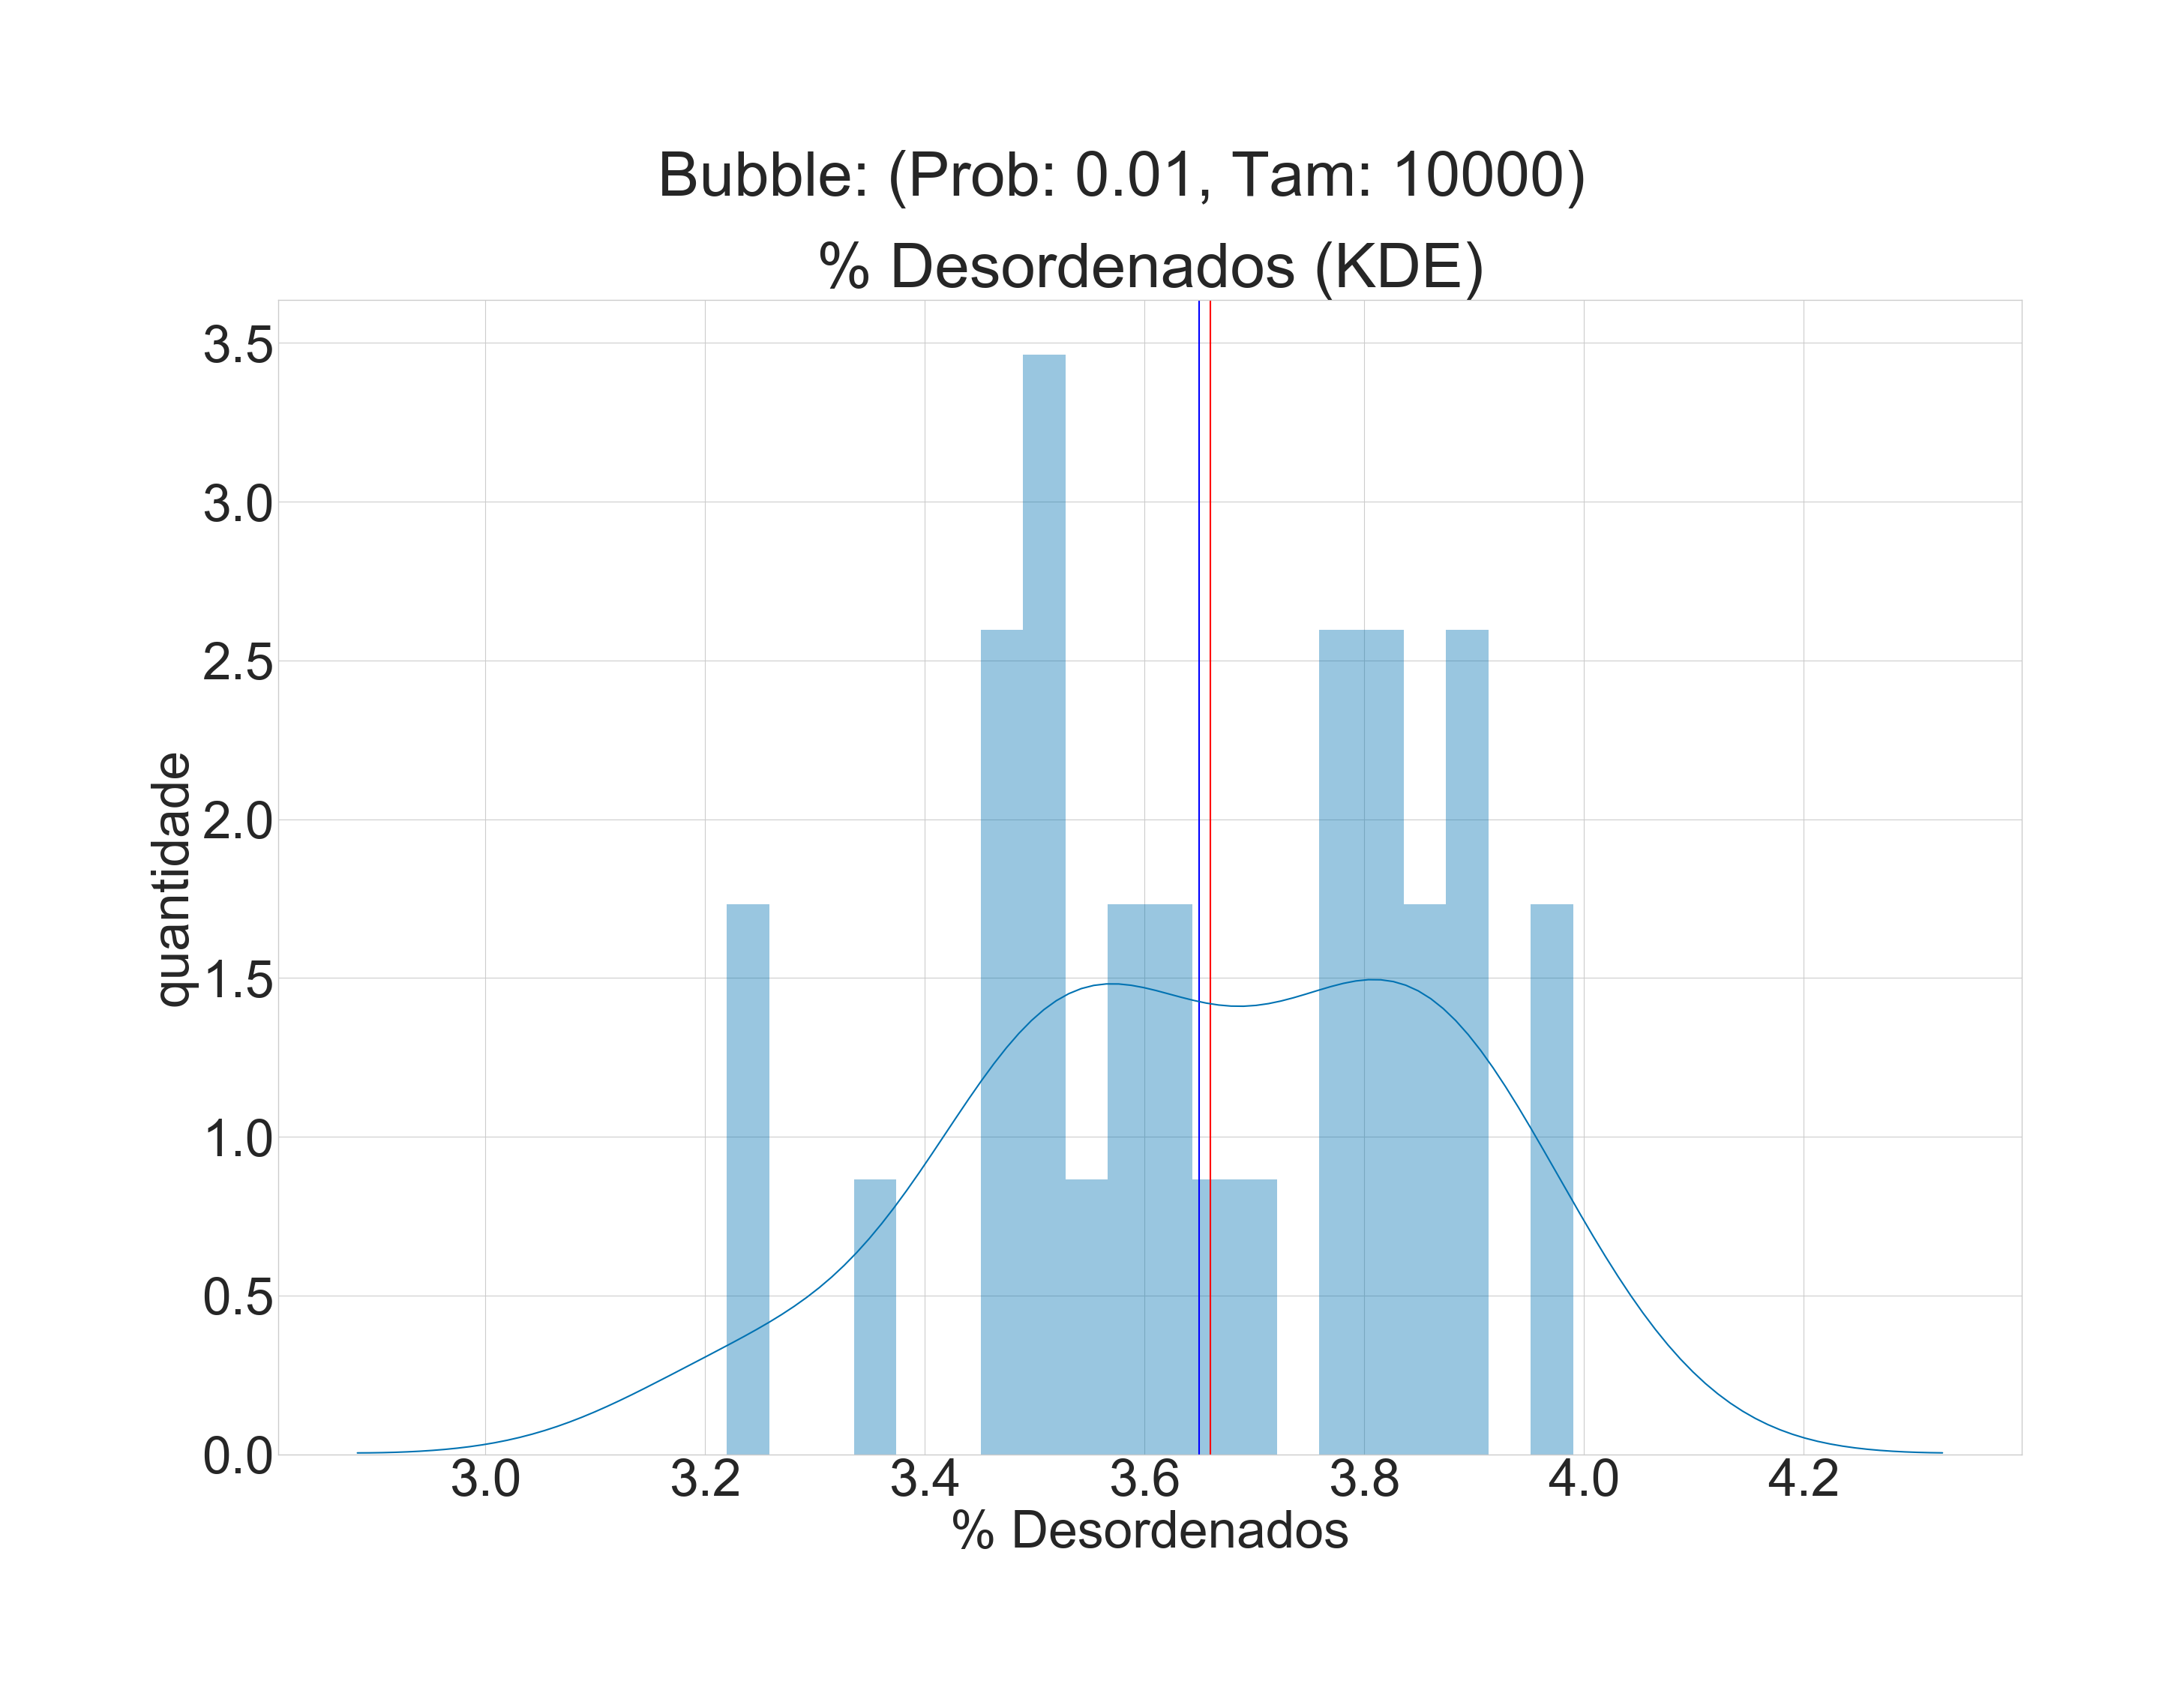
\includegraphics[scale=0.12]{figures/0_01_10000_Bubble_distribution_graph}}
     \textsf{\caption[Distribution Graph for bubblesort.]{Distribution Graph for bubblesort.\label{fig-dist-bubble-001-100}}}
     \end{subfigure}%
     \begin{subfigure}{.5\textwidth}
     \centering
     \frame{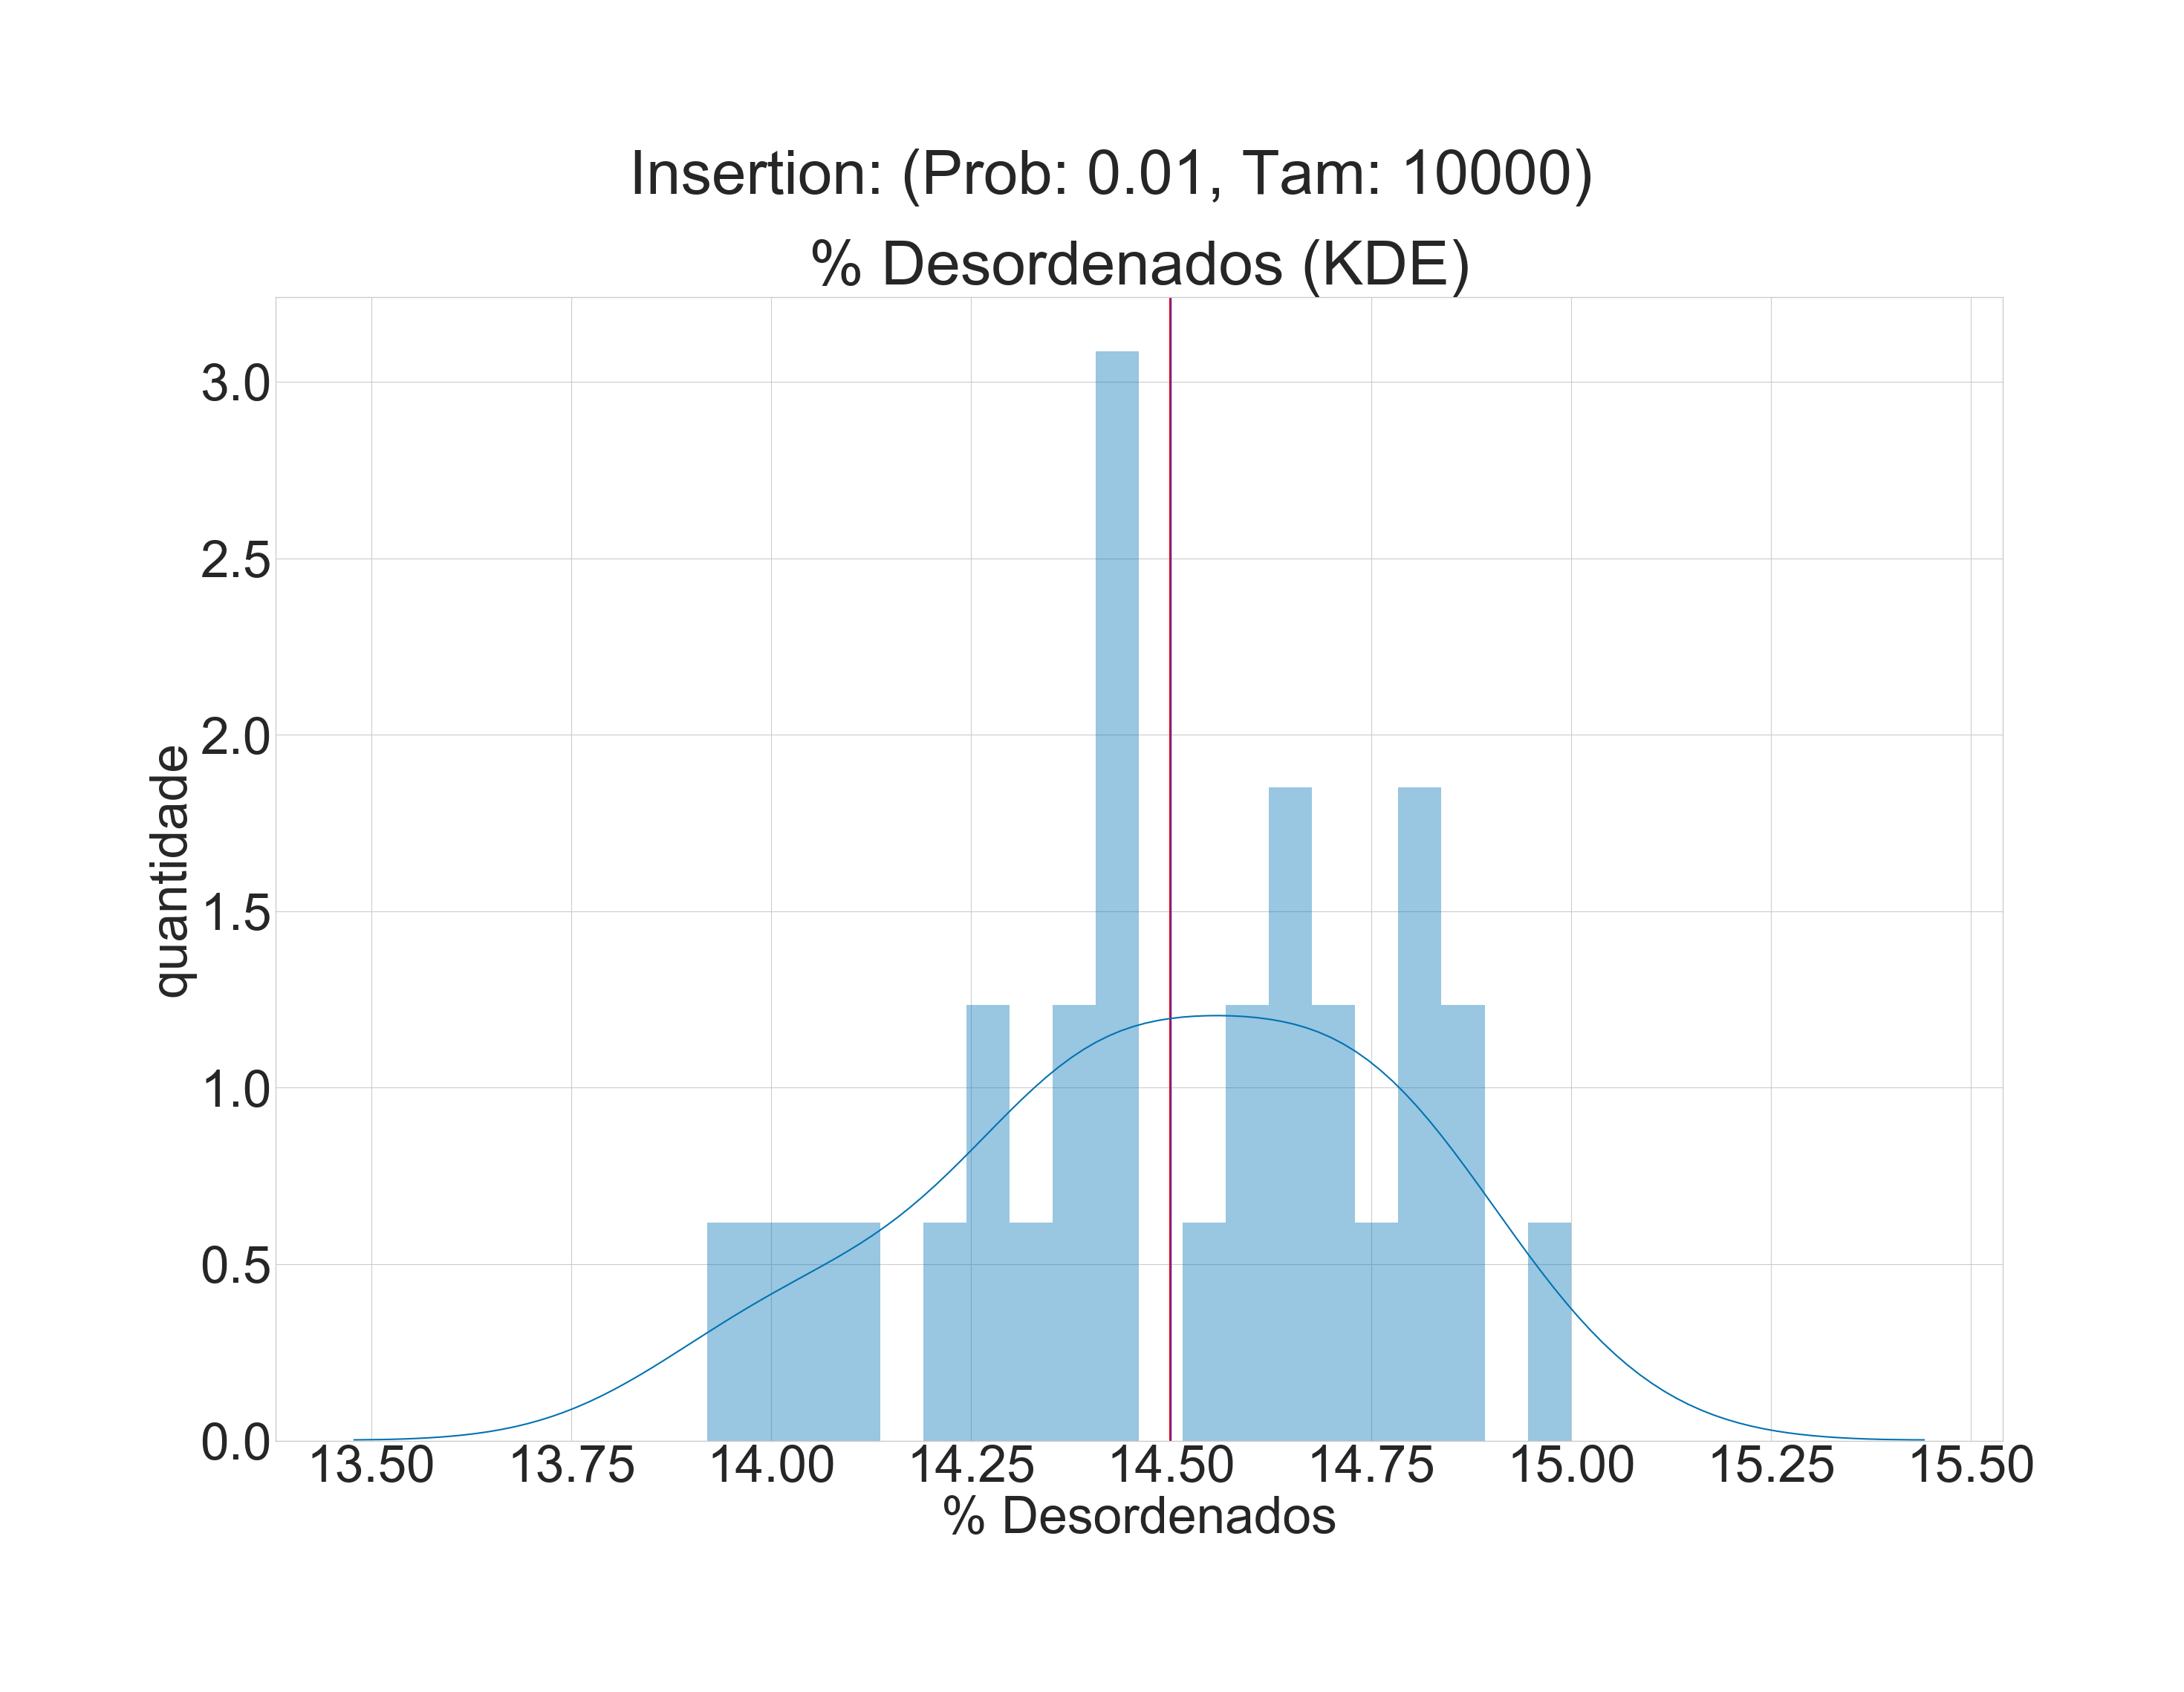
\includegraphics[scale=0.12]{figures/0_01_10000_Insertion_distribution_graph.png}}
     \textsf{\caption[Distribution Graph for insertion sort.]{Distribution Graph for insertion sort.\label{fig-dist-insertion-001-100}}}
     \end{subfigure}
     \begin{subfigure}{.5\textwidth}
     \centering
     \frame{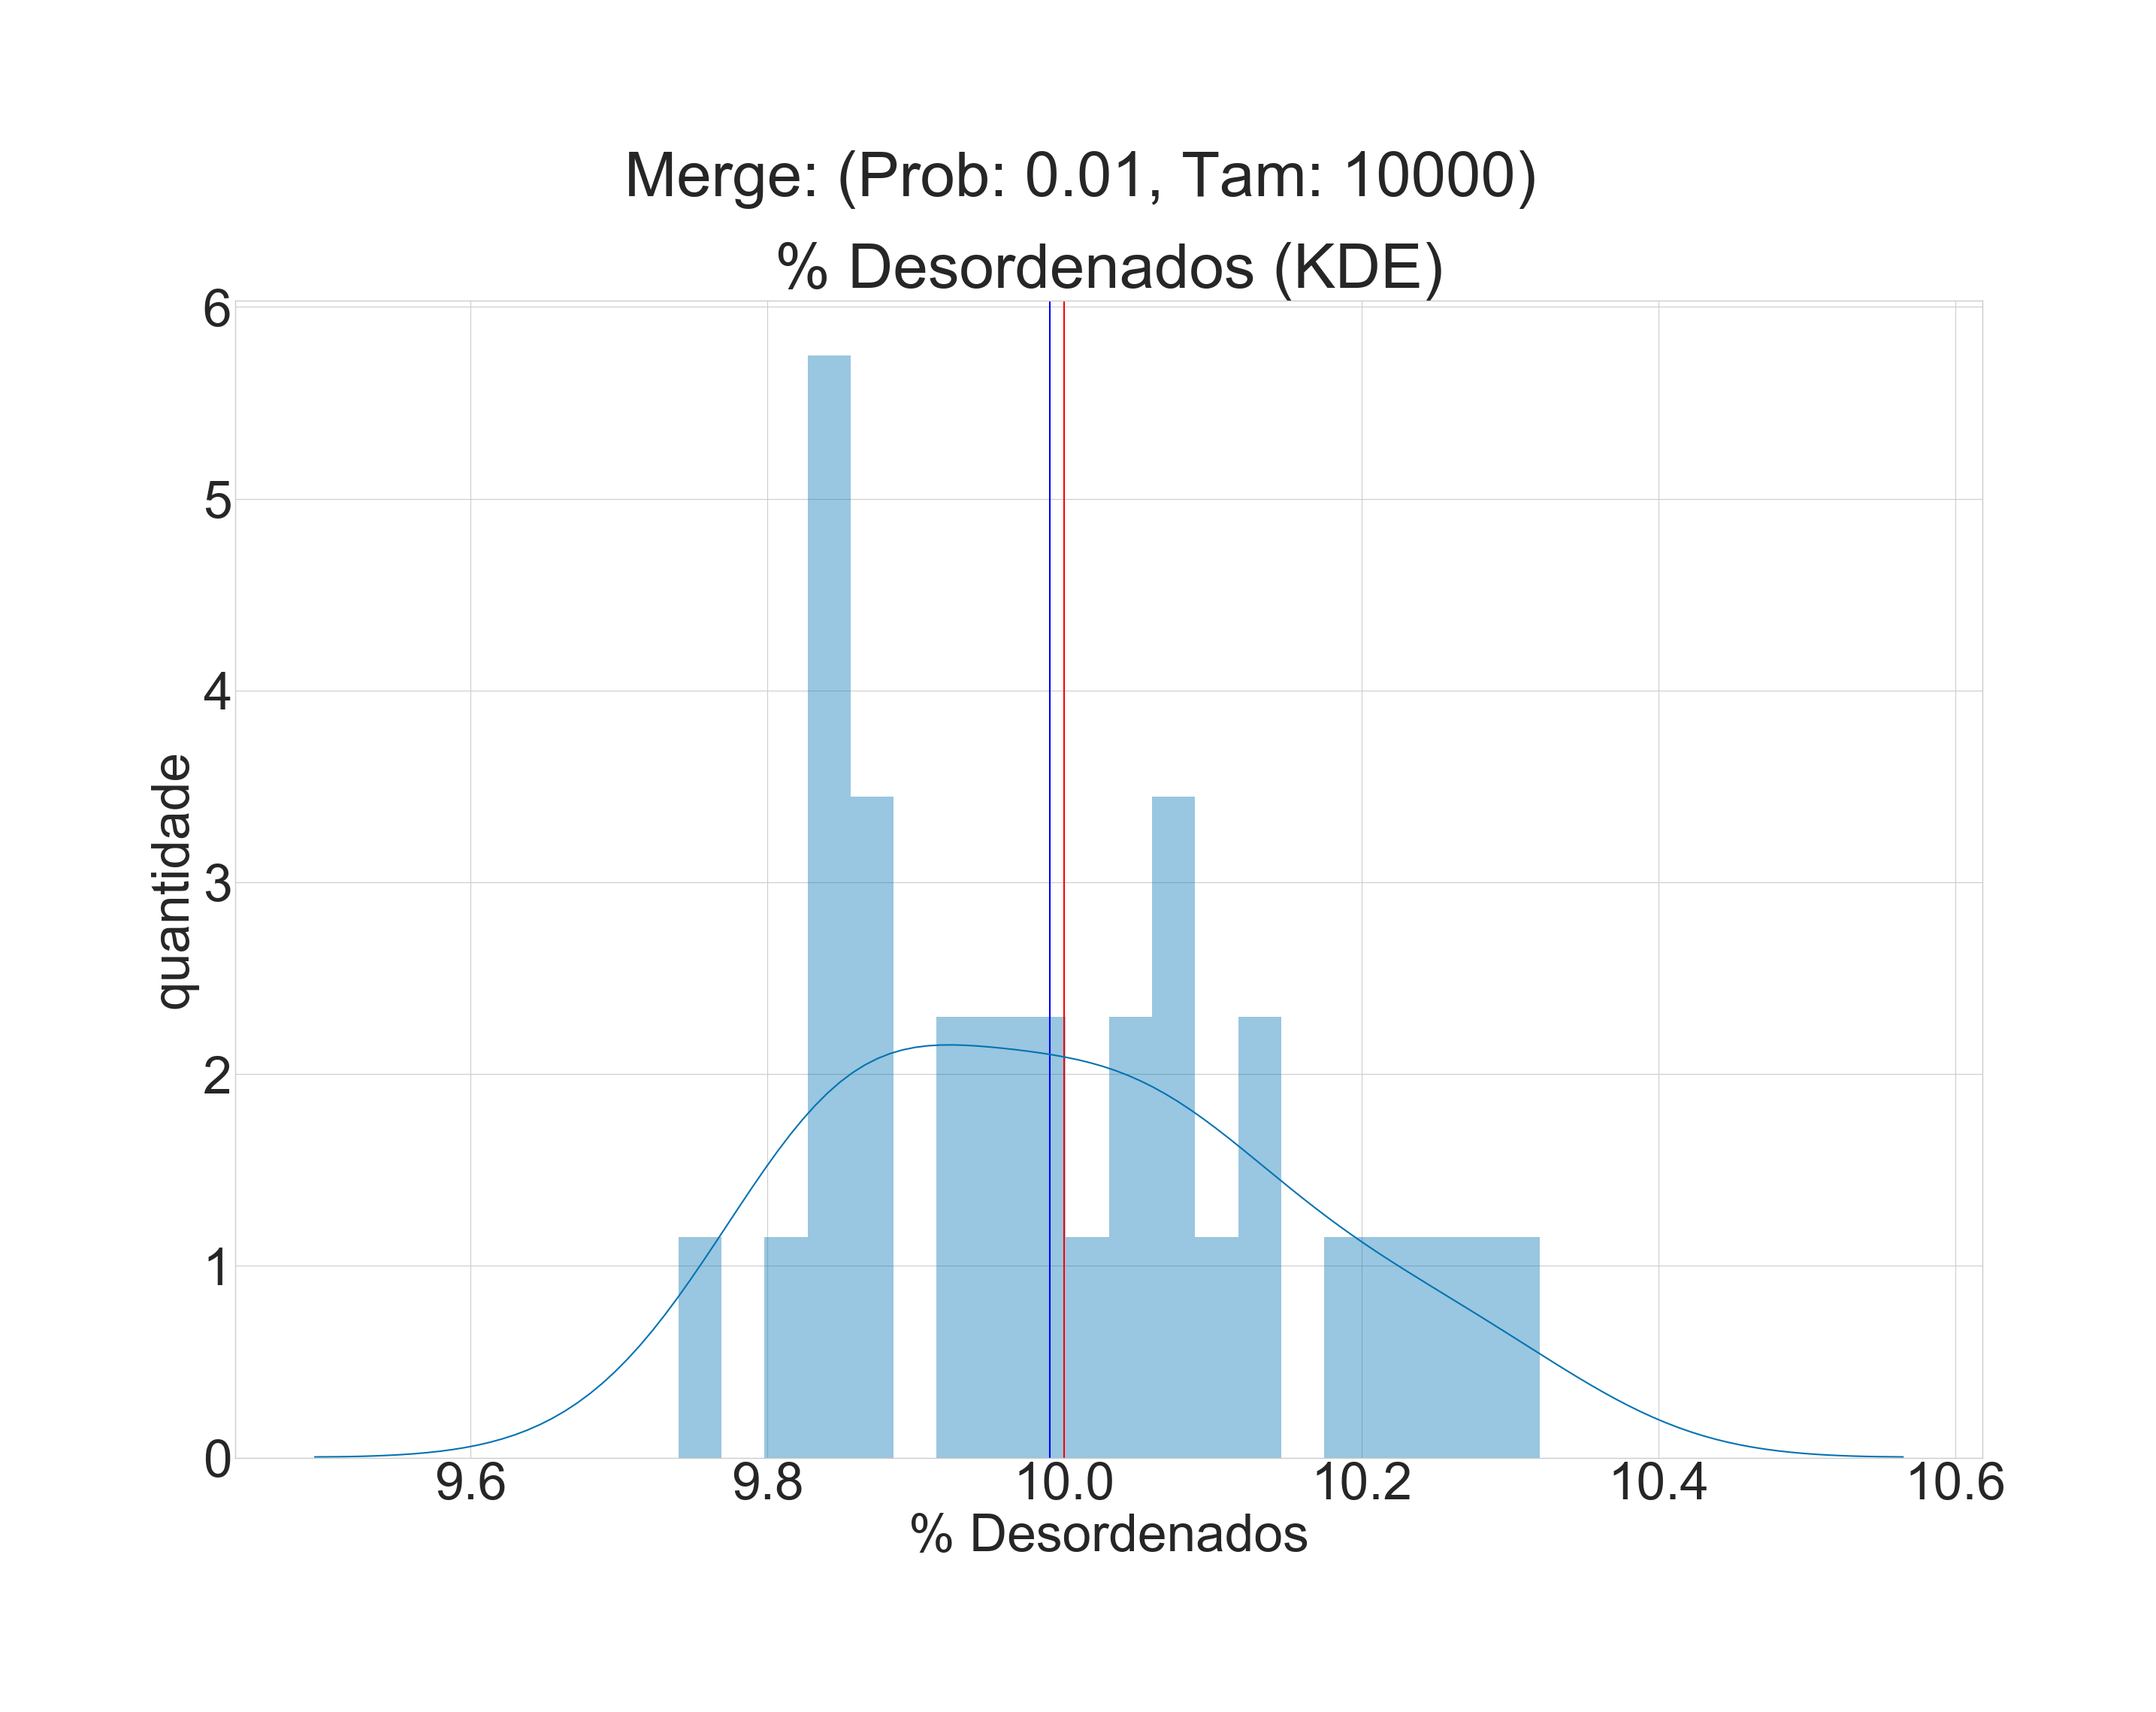
\includegraphics[scale=0.12]{figures/0_01_10000_Merge_distribution_graph.png}}
     \textsf{\caption[Distribution Graph for mergesort.]{Distribution Graph for mergesort.\label{fig-dist-merge-001-100}}}
     \end{subfigure}%
     \begin{subfigure}{.5\textwidth}
     \centering
     \frame{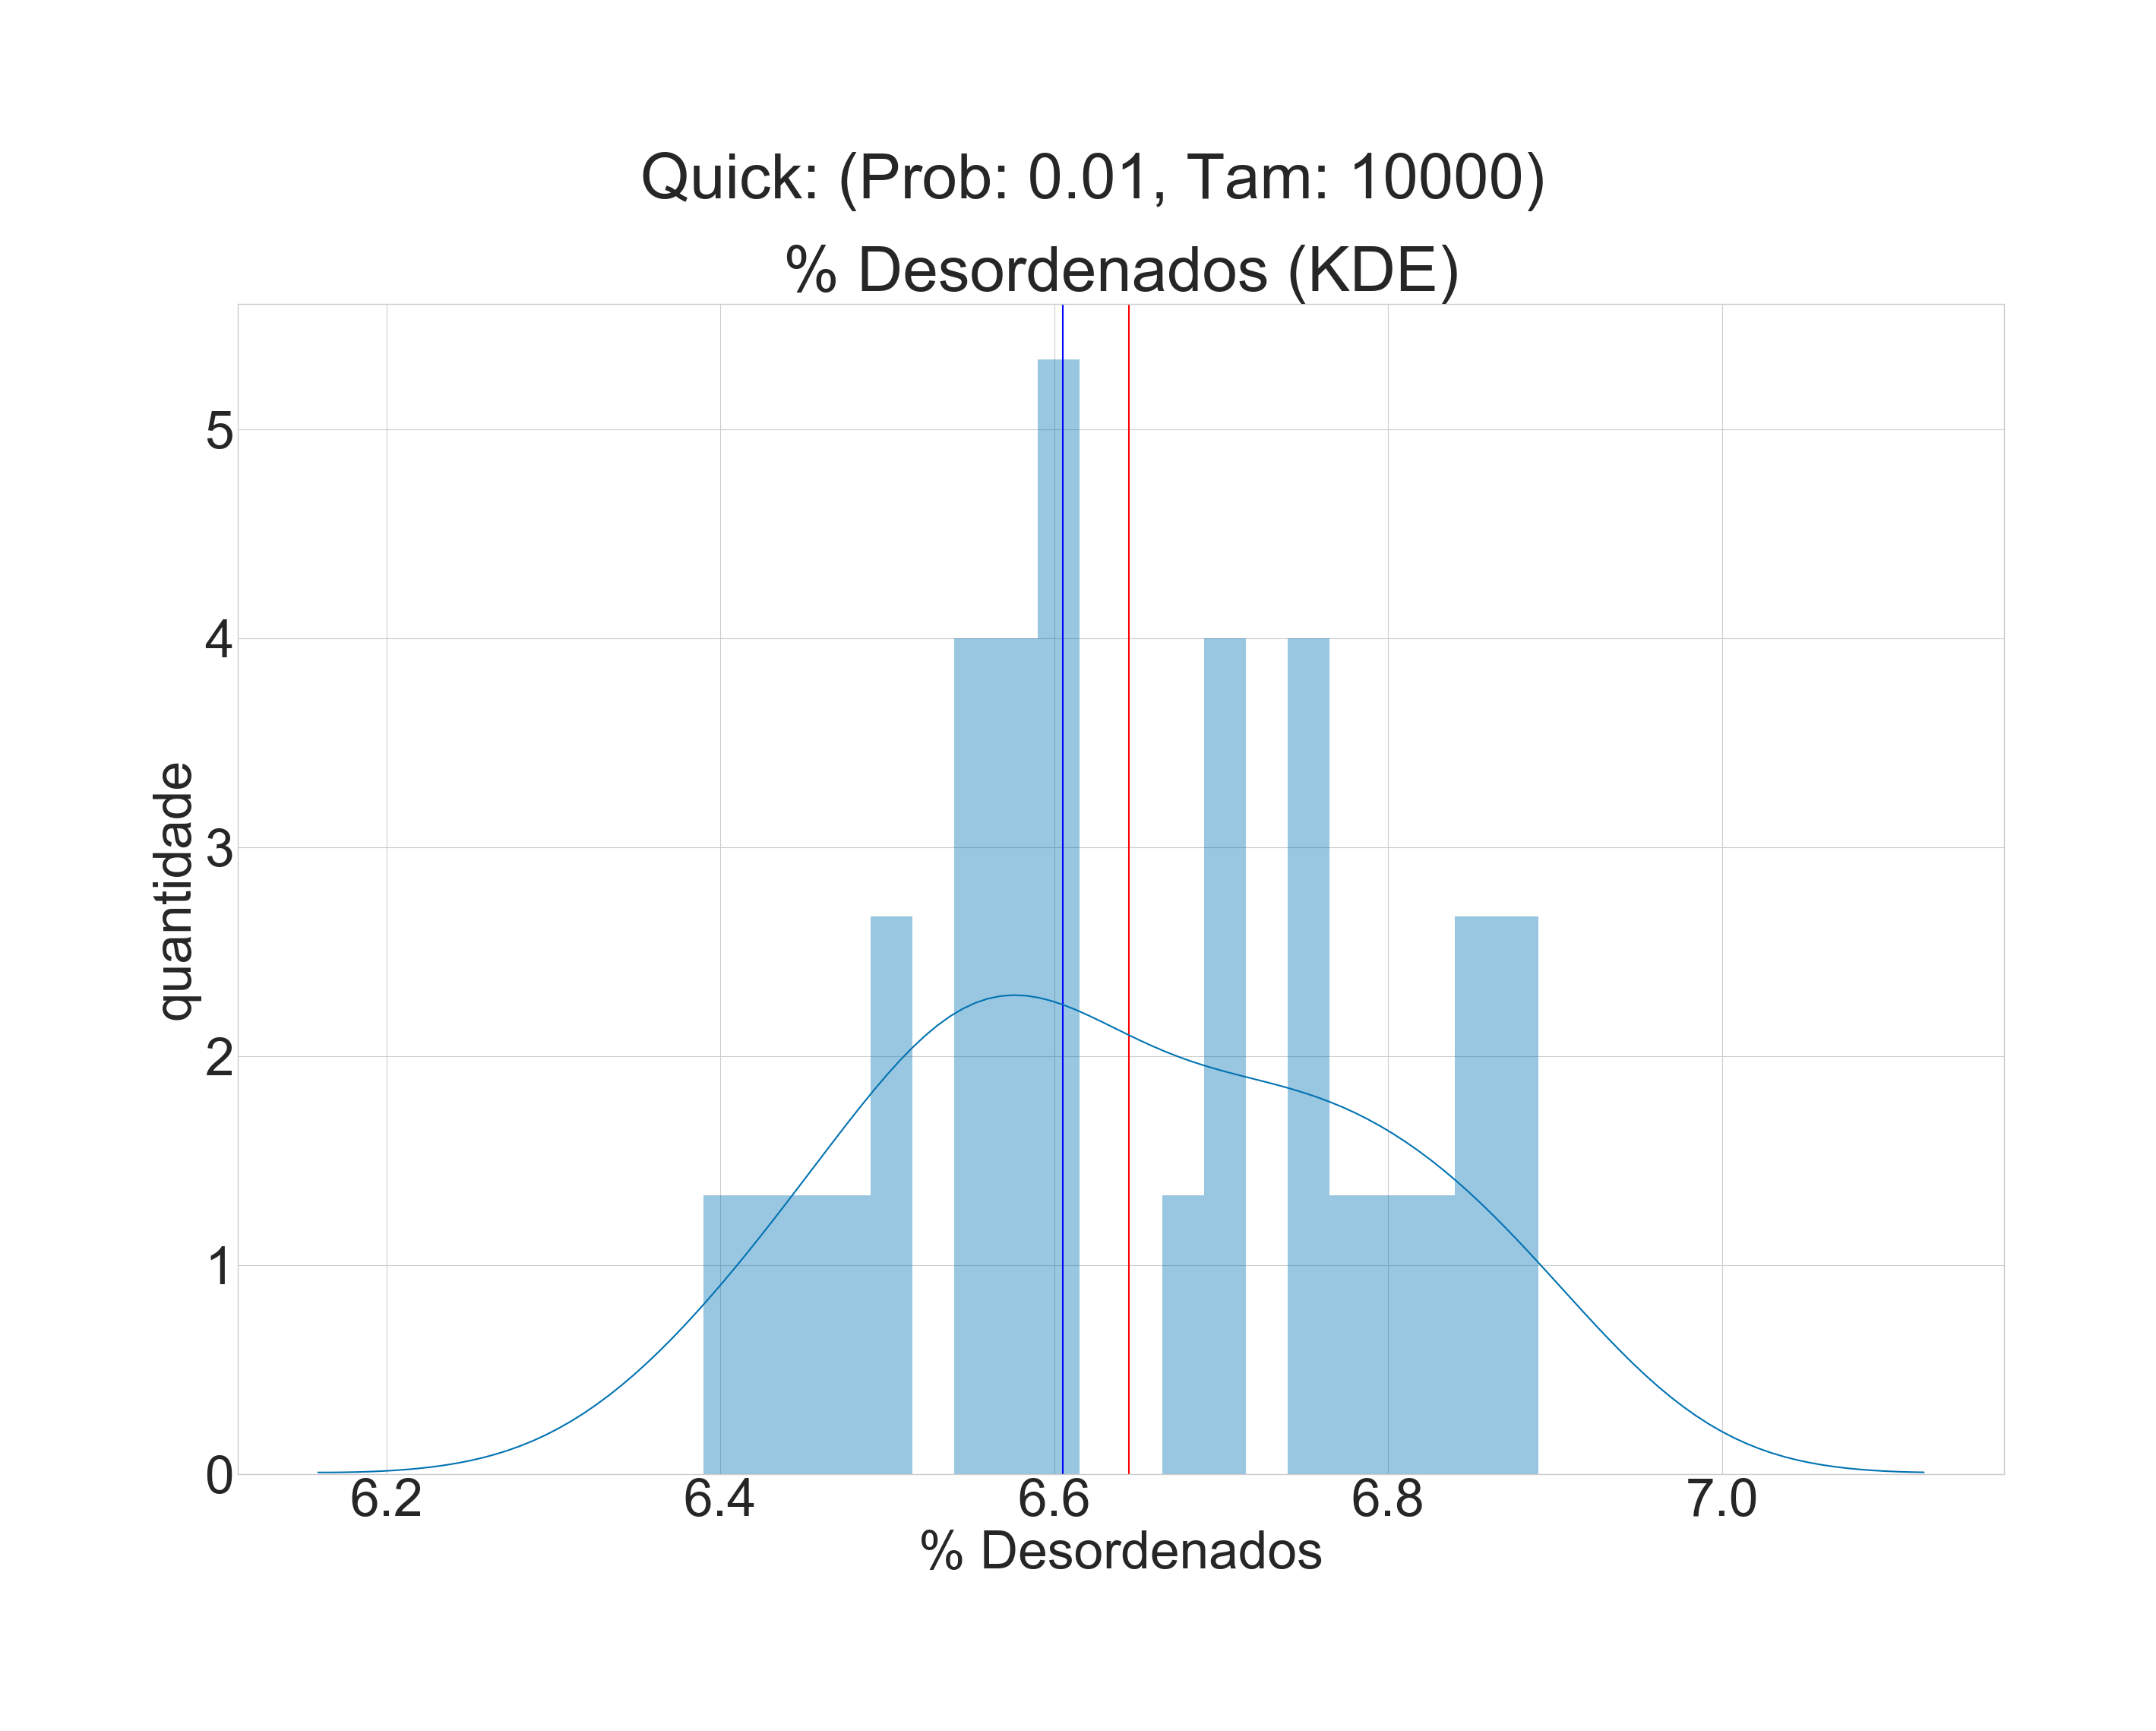
\includegraphics[scale=0.12]{figures/0_01_10000_Quick_distribution_graph.png}}
     \textsf{\caption[Distribution Graph for quicksort.]{Distribution Graph for quicksort.\label{fig-dist-quick-001-100}}}
     \end{subfigure}
     \caption{Distribution graph for a probability failure of 1\% and a sequence size of 10000.}
    \label{fig-distribution-graph}
\end{figure}

Q-Q plot shows that how much more blue points close to the red line, most normal is the distribution. Figure \ref{fig-qqplot} below presents this graph for a probability failure of 1\% and a sequence size of 10000 for considered sorting algorithms.

\begin{figure}[H]
    \centering
    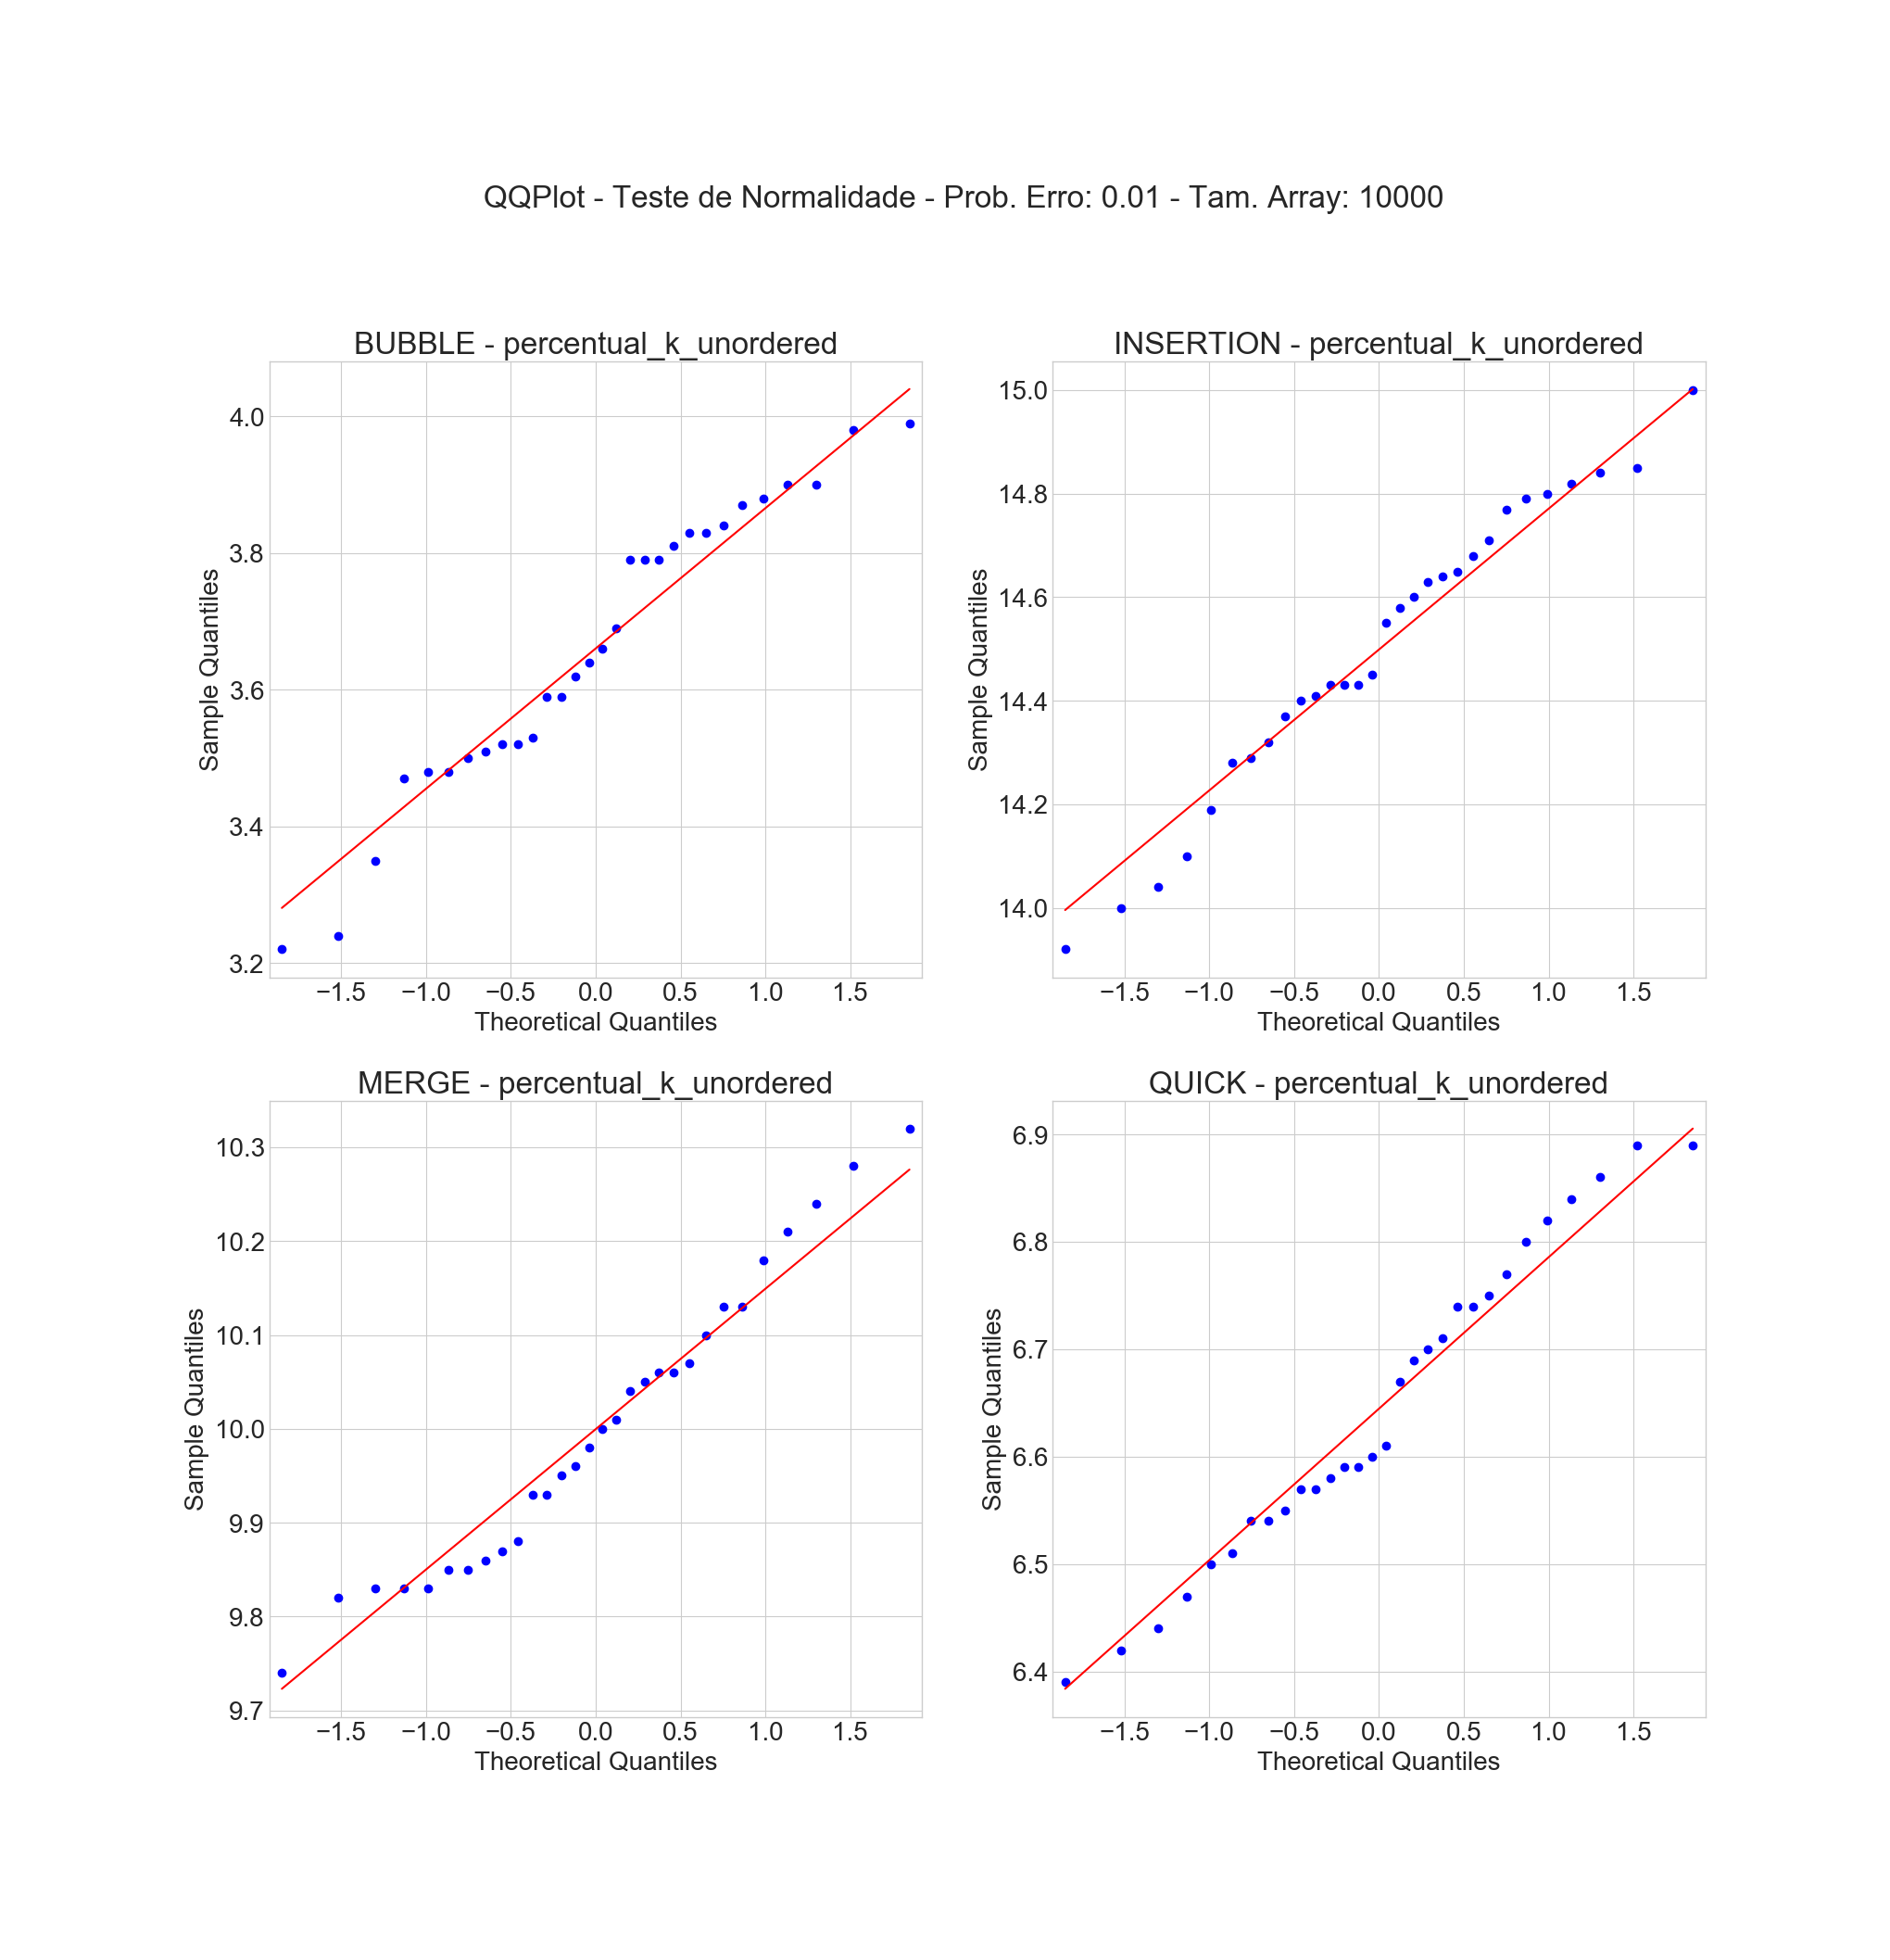
\includegraphics[scale=0.37]{figures/anova_prob_0_01_tam_10000_DESORDENADOS_PERCENTUAL.png}
    \textsf{\caption[Q-Q plot showing normal distribution for a probability failure of 1\% and a sequence size of 10000.]{Q-Q plot showing normal distribution for a probability failure of 1\% and a sequence size of 10000.\label{fig-qqplot}}}
 \end{figure}

\subsection{Conclusions}



\section{Results}

\section{Discussion}

\section{Conclusion}

This work proposes a study and discussion of how sorting algorithms, particularly Quicksort, Mergesort, Insertion Sort, and Bubblesort, are affected by memory faults. To achieve this, we define the experimental setup, showing the dependent and independent variables, then the used dataset with its characteristics. Next, we performed data analysis after the execution of sorting algorithms over the dataset. As explained in this work, we analyzed only the dependent variables \textit{percentage of the largest subarray size ((\%LSS)} and \textit{percentage of unordered elements quantity (\%UEQ)}. These variables, because they are a percentage value, already were normalized (i.e., the same order of magnitude) related to dependent variable \textit{array size}.

We ran a normality test and, after that, we determined that only the dependent variable \%UEQ (\textit{percentage of unordered elements quantity}) has a normal distribution related to mean for all algorithms, so we choosed to test just the hypothesis associated with the dependent variable \%UEQ.

After data analysis and discussion, we can conclude that, in this experiment, the worse algorithm related to \%UEQ variable was Insertion sort. This algorithm had the highest mean values in almost all combinations of study. These values were much higher than other algorithms when tested with \textit{probability of failure} of 1\% (0.01). Finally, our tests shows that, in general, Quicksort algorithm was better than Mergesort.

For linear regression, our results showed that for dependent variable \%UEQ variable we get a linear model that explains at least 80\% of relation between this variable and indepentent variable probability of failure.

We can, then, with our results, elaborate a ranking of the performance of algorithms when considering memory faults:
\begin{enumerate}
    \item Bubblesort
    \item Quicksort
    \item Mergesort
    \item Insertion sort
\end{enumerate}

All data used for this work can be downloaded at \href{https://bit.ly/392LZKR}{https://bit.ly/392LZKR}.

\section{Prepare Your Paper Before Styling}
Before you begin to format your paper, first write and save the content as a 
separate text file. Complete all content and organizational editing before 
formatting. Please note sections \ref{AA}--\ref{SCM} below for more information on 
proofreading, spelling and grammar.

Keep your text and graphic files separate until after the text has been 
formatted and styled. Do not number text heads---{\LaTeX} will do that 
for you.

\subsection{Abbreviations and Acronyms}\label{AA}
Define abbreviations and acronyms the first time they are used in the text, 
even after they have been defined in the abstract. Abbreviations such as 
IEEE, SI, MKS, CGS, ac, dc, and rms do not have to be defined. Do not use 
abbreviations in the title or heads unless they are unavoidable.

\subsection{Units}
\begin{itemize}
\item Use either SI (MKS) or CGS as primary units. (SI units are encouraged.) English units may be used as secondary units (in parentheses). An exception would be the use of English units as identifiers in trade, such as ``3.5-inch disk drive''.
\item Avoid combining SI and CGS units, such as current in amperes and magnetic field in oersteds. This often leads to confusion because equations do not balance dimensionally. If you must use mixed units, clearly state the units for each quantity that you use in an equation.
\item Do not mix complete spellings and abbreviations of units: ``Wb/m\textsuperscript{2}'' or ``webers per square meter'', not ``webers/m\textsuperscript{2}''. Spell out units when they appear in text: ``. . . a few henries'', not ``. . . a few H''.
\item Use a zero before decimal points: ``0.25'', not ``.25''. Use ``cm\textsuperscript{3}'', not ``cc''.)
\end{itemize}

\subsection{Equations}
Number equations consecutively. To make your 
equations more compact, you may use the solidus (~/~), the exp function, or 
appropriate exponents. Italicize Roman symbols for quantities and variables, 
but not Greek symbols. Use a long dash rather than a hyphen for a minus 
sign. Punctuate equations with commas or periods when they are part of a 
sentence, as in:
\begin{equation}
a+b=\gamma\label{eq}
\end{equation}

Be sure that the 
symbols in your equation have been defined before or immediately following 
the equation. Use ``\eqref{eq}'', not ``Eq.~\eqref{eq}'' or ``equation \eqref{eq}'', except at 
the beginning of a sentence: ``Equation \eqref{eq} is . . .''

\subsection{\LaTeX-Specific Advice}

Please use ``soft'' (e.g., \verb|\eqref{Eq}|) cross references instead
of ``hard'' references (e.g., \verb|(1)|). That will make it possible
to combine sections, add equations, or change the order of figures or
citations without having to go through the file line by line.

Please don't use the \verb|{eqnarray}| equation environment. Use
\verb|{align}| or \verb|{IEEEeqnarray}| instead. The \verb|{eqnarray}|
environment leaves unsightly spaces around relation symbols.

Please note that the \verb|{subequations}| environment in {\LaTeX}
will increment the main equation counter even when there are no
equation numbers displayed. If you forget that, you might write an
article in which the equation numbers skip from (17) to (20), causing
the copy editors to wonder if you've discovered a new method of
counting.

{\BibTeX} does not work by magic. It doesn't get the bibliographic
data from thin air but from .bib files. If you use {\BibTeX} to produce a
bibliography you must send the .bib files. 

{\LaTeX} can't read your mind. If you assign the same label to a
subsubsection and a table, you might find that Table I has been cross
referenced as Table IV-B3. 

{\LaTeX} does not have precognitive abilities. If you put a
\verb|\label| command before the command that updates the counter it's
supposed to be using, the label will pick up the last counter to be
cross referenced instead. In particular, a \verb|\label| command
should not go before the caption of a figure or a table.

Do not use \verb|\nonumber| inside the \verb|{array}| environment. It
will not stop equation numbers inside \verb|{array}| (there won't be
any anyway) and it might stop a wanted equation number in the
surrounding equation.

\subsection{Some Common Mistakes}\label{SCM}
\begin{itemize}
\item The word ``data'' is plural, not singular.
\item The subscript for the permeability of vacuum $\mu_{0}$, and other common scientific constants, is zero with subscript formatting, not a lowercase letter ``o''.
\item In American English, commas, semicolons, periods, question and exclamation marks are located within quotation marks only when a complete thought or name is cited, such as a title or full quotation. When quotation marks are used, instead of a bold or italic typeface, to highlight a word or phrase, punctuation should appear outside of the quotation marks. A parenthetical phrase or statement at the end of a sentence is punctuated outside of the closing parenthesis (like this). (A parenthetical sentence is punctuated within the parentheses.)
\item A graph within a graph is an ``inset'', not an ``insert''. The word alternatively is preferred to the word ``alternately'' (unless you really mean something that alternates).
\item Do not use the word ``essentially'' to mean ``approximately'' or ``effectively''.
\item In your paper title, if the words ``that uses'' can accurately replace the word ``using'', capitalize the ``u''; if not, keep using lower-cased.
\item Be aware of the different meanings of the homophones ``affect'' and ``effect'', ``complement'' and ``compliment'', ``discreet'' and ``discrete'', ``principal'' and ``principle''.
\item Do not confuse ``imply'' and ``infer''.
\item The prefix ``non'' is not a word; it should be joined to the word it modifies, usually without a hyphen.
\item There is no period after the ``et'' in the Latin abbreviation ``et al.''.
\item The abbreviation ``i.e.'' means ``that is'', and the abbreviation ``e.g.'' means ``for example''.
\end{itemize}
An excellent style manual for science writers is \cite{b7}.

\subsection{Authors and Affiliations}
\textbf{The class file is designed for, but not limited to, six authors.} A 
minimum of one author is required for all conference articles. Author names 
should be listed starting from left to right and then moving down to the 
next line. This is the author sequence that will be used in future citations 
and by indexing services. Names should not be listed in columns nor group by 
affiliation. Please keep your affiliations as succinct as possible (for 
example, do not differentiate among departments of the same organization).

\subsection{Identify the Headings}
Headings, or heads, are organizational devices that guide the reader through 
your paper. There are two types: component heads and text heads.

Component heads identify the different components of your paper and are not 
topically subordinate to each other. Examples include Acknowledgments and 
References and, for these, the correct style to use is ``Heading 5''. Use 
``figure caption'' for your Figure captions, and ``table head'' for your 
table title. Run-in heads, such as ``Abstract'', will require you to apply a 
style (in this case, italic) in addition to the style provided by the drop 
down menu to differentiate the head from the text.

Text heads organize the topics on a relational, hierarchical basis. For 
example, the paper title is the primary text head because all subsequent 
material relates and elaborates on this one topic. If there are two or more 
sub-topics, the next level head (uppercase Roman numerals) should be used 
and, conversely, if there are not at least two sub-topics, then no subheads 
should be introduced.

\subsection{Figures and Tables}
\paragraph{Positioning Figures and Tables} Place figures and tables at the top and 
bottom of columns. Avoid placing them in the middle of columns. Large 
figures and tables may span across both columns. Figure captions should be 
below the figures; table heads should appear above the tables. Insert 
figures and tables after they are cited in the text. Use the abbreviation 
``Fig.~\ref{fig}'', even at the beginning of a sentence.

\begin{table}[htbp]
\caption{Table Type Styles}
\begin{center}
\begin{tabular}{|c|c|c|c|}
\hline
\textbf{Table}&\multicolumn{3}{|c|}{\textbf{Table Column Head}} \\
\cline{2-4} 
\textbf{Head} & \textbf{\textit{Table column subhead}}& \textbf{\textit{Subhead}}& \textbf{\textit{Subhead}} \\
\hline
copy& More table copy$^{\mathrm{a}}$& &  \\
\hline
\multicolumn{4}{l}{$^{\mathrm{a}}$Sample of a Table footnote.}
\end{tabular}
\label{tab1}
\end{center}
\end{table}

% \begin{figure}[htbp]
% \centerline{\includegraphics{fig1.png}}
% \caption{Example of a figure caption.}
% \label{fig}
% \end{figure}

Figure Labels: Use 8 point Times New Roman for Figure labels. Use words 
rather than symbols or abbreviations when writing Figure axis labels to 
avoid confusing the reader. As an example, write the quantity 
``Magnetization'', or ``Magnetization, M'', not just ``M''. If including 
units in the label, present them within parentheses. Do not label axes only 
with units. In the example, write ``Magnetization (A/m)'' or ``Magnetization 
\{A[m(1)]\}'', not just ``A/m''. Do not label axes with a ratio of 
quantities and units. For example, write ``Temperature (K)'', not 
``Temperature/K''.

\section*{Acknowledgment}

The preferred spelling of the word ``acknowledgment'' in America is without 
an ``e'' after the ``g''. Avoid the stilted expression ``one of us (R. B. 
G.) thanks $\ldots$''. Instead, try ``R. B. G. thanks$\ldots$''. Put sponsor 
acknowledgments in the unnumbered footnote on the first page.

\bibliography{RM1_Assignment}
\bibliographystyle{ieeetr}

\end{document}